

\section{Prueba 5}

\subsection{Red de inferencia}
\begin{center}
	\tikzstyle{regla}= [rectangle,draw,black,fill=blue!15]
	\tikzstyle{hecho}= [rectangle,draw,black,fill=black!15]
	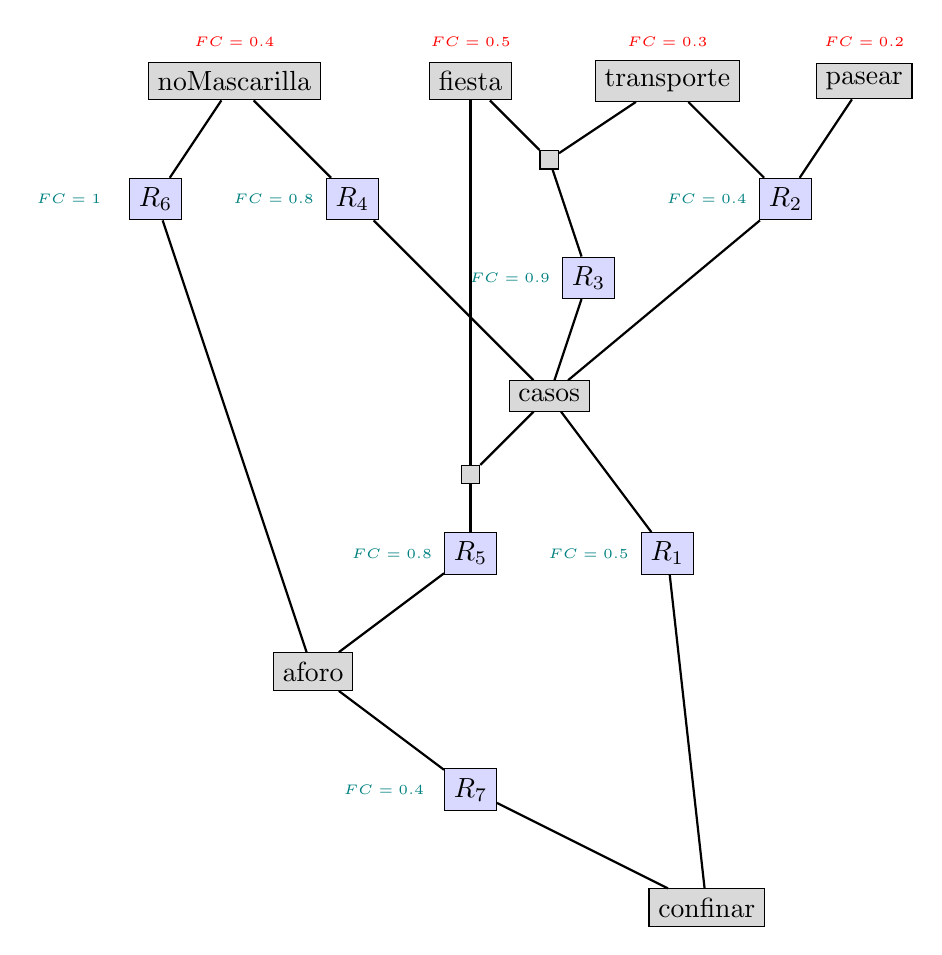
\begin{tikzpicture}
		
		\node (a) at (-4,5) [hecho] {noMascarilla};
		\node at (-4,5.5) {\color{red}{\tiny{$FC=0.4$}}};

		\node (b) at (-1,5) [hecho] {fiesta};
        \node at (-1,5.5) {\color{red}{\tiny{$FC=0.5$}}};

		\node (c) at (1.5,5) [hecho] {transporte};
		\node at (1.5,5.5) {\color{red}{\tiny{$FC=0.3$}}};

		\node (d) at (4,5)[hecho] {pasear};
        \node at (4,5.5) {\color{red}{\tiny{$FC=0.2$}}};

		\node (e) at (0,1)[hecho] {casos};
		
		\node (f) at (-3,-2.5)[hecho] {aforo};

        \node (g) at (2,-5.5)[hecho] {confinar};

		\node (b/c) at (0,4)[hecho] {};
        \node (b/e) at (-1,0)[hecho] {};

		\node (r1) at (1.5,-1) [regla] {$R_{1}$};
		\node at (0.5,-1) {\color{teal}{\tiny{$FC=0.5$}}};
		\node (r2) at (3,3.5) [regla] {$R_{2}$};
		\node at (2,3.5) {\color{teal}{\tiny{$FC=0.4$}}};
		\node (r3) at (0.5,2.5) [regla] {$R_{3}$};
		\node at (-0.5, 2.5) {\color{teal}{\tiny{$FC=0.9$}}};
		\node (r4) at (-2.5,3.5) [regla] {$R_{4}$};
		\node at (-3.5,3.5) {\color{teal}{\tiny{$FC=0.8$}}};
		\node (r5) at (-1,-1) [regla] {$R_{5}$};
		\node at (-2,-1) {\color{teal}{\tiny{$FC=0.8$}}};
		\node (r6) at (-5,3.5) [regla] {$R_{6}$};
		\node at (-6.1,3.5) {\color{teal}{\tiny{$FC=1$}}};
        \node (r7) at (-1,-4) [regla] {$R_{7}$};
		\node at (-2.1,-4) {\color{teal}{\tiny{$FC=0.4$}}};
		
		\path[black,thick] (a) edge[] node {} (r4);
        \path[black,thick] (r4) edge[] node {} (e);
        \path[black,thick] (e) edge[] node {} (b/e);
        \path[black,thick] (b/e) edge[] node {} (r5);
        \path[black,thick] (r5) edge[] node {} (f);
        \path[black,thick] (r6) edge[] node {} (f);
        \path[black,thick] (f) edge[] node {} (r7);

        \path[black,thick] (e) edge[] node {} (r1);
        \path[black,thick] (r1) edge[] node {} (g);
        \path[black,thick] (g) edge[] node {} (r7);
        \path[black,thick] (a) edge[] node {} (r6);

        \path[black,thick] (b) edge[] node {} (b/e);
        \path[black,thick] (b) edge[] node {} (b/c);
        \path[black,thick] (c) edge[] node {} (b/c);
        \path[black,thick] (b/c) edge[] node {} (r3);
        \path[black,thick] (r3) edge[] node {} (e);

        \path[black,thick] (c) edge[] node {} (r2);
        \path[black,thick] (d) edge[] node {} (r2);
        \path[black,thick] (r2) edge[] node {} (e);
	\end{tikzpicture}
\end{center}

\break

\par Esta red de inferencia se debe interpretar de arriba a abajo.
Los rectángulos azules son las reglas, los grises que están ligados por encima 
de ellas son sus antecedentes, si estos antecedentes convergen en un cuadrado 
quiere decir que es la conjunción de esos literales, en caso contrario son disyunciones
o simplemente un literal. Los rectángulos grises que cuelgan de las reglas 
son sus consecuentes respectivamente. Además, incluyo los factores de certeza propocionados por
la Base de hechos y la Base de Conocimiento iniciales.
\subsection{Proceso de inferencia}
\begin{listing}[language=Pascal]
(Razonamiento dirigido por Metas)
Objetivo: confinar
Proceso de Inferencia: 
  ###########################
  # Llamada (1) a verificar #
  ###########################
	Verificar(confinar,{fiesta,noMascarilla,pasear,
	transporte}) // Recursion 
	Conjunto Conflicto={R1,R7} // confinar es consecuente de estas reglas
	R={R1} // Seleccionar regla R1
	Eliminar R1 ---> Conjunto Conflicto={R7,}
	NuevasMetas={casos} // Antecedentes de R1; Verificado = true
	Meta=casos // Seleccionar casos de NuevasMetas
	NuevasMetas={} // Eliminar casos de NuevasMetas
  ###########################
  # Llamada (2) a verificar #
  ###########################
	Verificar(casos,{fiesta,noMascarilla,pasear,
	transporte}) // Recursion 
	Conjunto Conflicto={R2,R3,R4} // casos es consecuente de estas reglas
	R={R2} // Seleccionar regla R2
	Eliminar R2 ---> Conjunto Conflicto={R3,R4}
	NuevasMetas={pasear,transporte} // Antecedentes de R2; Verificado = true
	Meta=pasear // Seleccionar pasear de NuevasMetas
	NuevasMetas={transporte} // Eliminar pasear de NuevasMetas
  ###########################
  # Llamada (3) a verificar #
  ###########################
	Verificar(pasear,{fiesta,noMascarilla,pasear,
	transporte}) ---> true // Recursion: pasear en BH
	BH={fiesta,noMascarilla,pasear,transporte}
	Meta=transporte // Seleccionar transporte de NuevasMetas
	NuevasMetas={} // Eliminar transporte de NuevasMetas
  ###########################
  # Llamada (4) a verificar #
  ###########################
	Verificar(transporte,{fiesta,noMascarilla,pasear,
	transporte}) ---> true // Recursion: transporte en BH
	BH={fiesta,noMascarilla,pasear,transporte}
	(CASO 1): Combinacion de antecedentes de R2
	 FC(transporte o pasear)=min(FC(pasear),FC(transporte))=0.3
	(CASO 3): Combinacion de la evidencia con la regla R2
	 FC(casos{R2})=0.4*max(0,FC(transporte o pasear))=0.12
	Conjunto Conflicto={R3,R4} // casos es consecuente de estas reglas
	R={R3} // Seleccionar regla R3
	Eliminar R3 ---> Conjunto Conflicto={R4}
	NuevasMetas={fiesta,transporte} // Antecedentes de R3; Verificado = true
	Meta=fiesta // Seleccionar fiesta de NuevasMetas
	NuevasMetas={transporte} // Eliminar fiesta de NuevasMetas
  ###########################
  # Llamada (5) a verificar #
  ###########################
	Verificar(fiesta,{fiesta,noMascarilla,pasear,
	transporte}) ---> true // Recursion: fiesta en BH
	BH={fiesta,noMascarilla,pasear,transporte}
	Meta=transporte // Seleccionar transporte de NuevasMetas
	NuevasMetas={} // Eliminar transporte de NuevasMetas
  ###########################
  # Llamada (6) a verificar #
  ###########################
	Verificar(transporte,{fiesta,noMascarilla,pasear,
	transporte}) ---> true // Recursion: transporte en BH
	BH={fiesta,noMascarilla,pasear,transporte}
	(CASO 1): Combinacion de antecedentes de R3
	 FC(transporte y fiesta)=min(FC(fiesta),FC(transporte))=0.3
	(CASO 3): Combinacion de la evidencia con la regla R3
	 FC(casos{R3})=0.9*max(0,FC(transporte y fiesta))=0.27
	Conjunto Conflicto={R4} // casos es consecuente de estas reglas
	R={R4} // Seleccionar regla R4
	Eliminar R4 ---> Conjunto Conflicto={}
	NuevasMetas={noMascarilla} // Antecedentes de R4; Verificado = true
	Meta=noMascarilla // Seleccionar noMascarilla de NuevasMetas
	NuevasMetas={} // Eliminar noMascarilla de NuevasMetas
  ###########################
  # Llamada (7) a verificar #
  ###########################
	Verificar(noMascarilla,{fiesta,noMascarilla,pasear,
	transporte}) ---> true // Recursion: noMascarilla en BH
	BH={fiesta,noMascarilla,pasear,transporte}
	(CASO 1): Combinacion de antecedentes de R4
	 FC(noMascarilla)=min(FC(noMascarilla))=0.4
	(CASO 3): Combinacion de la evidencia con la regla R4
	 FC(casos{R4})=0.8*max(0,FC(noMascarilla))=0.32
	(CASO 2): Combinacion de las reglas R2 y R3
	 FC(casos)=FC(casos{R2}) + FC(casos{R3})*(1-FC(casos{R2}))=0.3576
	(CASO 2): Combinacion de las reglas R3 y R4
	 FC(casos)=FC(casos{R3}) + FC(casos{R4})*(1-FC(casos{R3}))=0.563168
	BH={casos,fiesta,noMascarilla,pasear,transporte} // Insertar casos a la Base de Hechos
	(CASO 1): Combinacion de antecedentes de R1
	 FC(casos)=min(FC(casos))=0.563168
	(CASO 3): Combinacion de la evidencia con la regla R1
	 FC(confinar{R1})=0.5*max(0,FC(casos))=0.281584
	Conjunto Conflicto={R7} // confinar es consecuente de estas reglas
	R={R7} // Seleccionar regla R7
	Eliminar R7 ---> Conjunto Conflicto={}
	NuevasMetas={aforo} // Antecedentes de R7; Verificado = true
	Meta=aforo // Seleccionar aforo de NuevasMetas
	NuevasMetas={} // Eliminar aforo de NuevasMetas
  ###########################
  # Llamada (8) a verificar #
  ###########################
	Verificar(aforo,{casos,fiesta,noMascarilla,pasear,
	transporte}) // Recursion 
	Conjunto Conflicto={R5,R6} // aforo es consecuente de estas reglas
	R={R5} // Seleccionar regla R5
	Eliminar R5 ---> Conjunto Conflicto={R6}
	NuevasMetas={casos,fiesta} // Antecedentes de R5; Verificado = true
	Meta=casos // Seleccionar casos de NuevasMetas
	NuevasMetas={fiesta} // Eliminar casos de NuevasMetas
  ###########################
  # Llamada (9) a verificar #
  ###########################
	Verificar(casos,{casos,fiesta,noMascarilla,pasear,
	transporte}) ---> true // Recursion: casos en BH
	BH={casos,fiesta,noMascarilla,pasear,transporte}
	Meta=fiesta // Seleccionar fiesta de NuevasMetas
	NuevasMetas={} // Eliminar fiesta de NuevasMetas
  ###########################
  # Llamada (10) a verificar #
  ###########################
	Verificar(fiesta,{casos,fiesta,noMascarilla,pasear,
	transporte}) ---> true // Recursion: fiesta en BH
	BH={casos,fiesta,noMascarilla,pasear,transporte}
	(CASO 1): Combinacion de antecedentes de R5
	 FC(fiesta y casos)=min(FC(casos),FC(fiesta))=0.5
	(CASO 3): Combinacion de la evidencia con la regla R5
	 FC(aforo{R5})=0.8*max(0,FC(fiesta y casos))=0.4
	Conjunto Conflicto={R6} // aforo es consecuente de estas reglas
	R={R6} // Seleccionar regla R6
	Eliminar R6 ---> Conjunto Conflicto={}
	NuevasMetas={noMascarilla} // Antecedentes de R6; Verificado = true
	Meta=noMascarilla // Seleccionar noMascarilla de NuevasMetas
	NuevasMetas={} // Eliminar noMascarilla de NuevasMetas
  ###########################
  # Llamada (11) a verificar #
  ###########################
	Verificar(noMascarilla,{casos,fiesta,noMascarilla,
	pasear,transporte}) ---> true // Recursion: noMascarilla en BH
	BH={casos,fiesta,noMascarilla,pasear,transporte}
	(CASO 1): Combinacion de antecedentes de R6
	 FC(noMascarilla)=min(FC(noMascarilla))=0.4
	(CASO 3): Combinacion de la evidencia con la regla R6
	 FC(aforo{R6})=1*max(0,FC(noMascarilla))=0.4
	(CASO 2): Combinacion de las reglas R5 y R6
	 FC(aforo)=FC(aforo{R5}) + FC(aforo{R6})*(1-FC(aforo{R5}))=0.64
	BH={aforo,casos,fiesta,noMascarilla,pasear,
	transporte} // Insertar aforo a la Base de Hechos
	(CASO 1): Combinacion de antecedentes de R7
	 FC(aforo)=min(FC(aforo))=0.64
	(CASO 3): Combinacion de la evidencia con la regla R7
	 FC(confinar{R7})=0.4*max(0,FC(aforo))=0.256
	(CASO 2): Combinacion de las reglas R1 y R7
	 FC(confinar)=FC(confinar{R1}) + FC(confinar{R7})*(1-FC(confinar{R1}))=0.465499
	BH={aforo,casos,confinar,fiesta,noMascarilla,pasear,
	transporte} // Insertar confinar a la Base de Hechos
Return TRUE
\end{listing}
\subsection{Objetivo obtenido por SBR-FC}
\begin{center}
\par -------------------- Hecho (confinar) ---------------------
\par Hecho (nomHecho): confinar
\par Hecho (facCerBH): 0.465499
\par ------------------------------------------------------------
\end{center}
